% RepNet Progress Update — Finalized Model Performance
% Same visual identity as final_presentation_modern.tex
% Compiles with pdfLaTeX.

\documentclass[10pt,aspectratio=169]{beamer}

% ====================
% Packages
% ====================
\usepackage[T1]{fontenc}
\usepackage{lmodern}
\usepackage{graphicx}
\usepackage{booktabs}
\usepackage{mathtools}
\usepackage{tikz}
\usetikzlibrary{positioning,arrows.meta}
\usepackage{hyperref}
\usepackage{pgfplots}
\pgfplotsset{compat=1.18}

% ====================
% UC Davis brand colors (digital palette)
% ====================
\definecolor{aggieblue}{HTML}{022851}
\definecolor{aggiegold}{HTML}{FFBF00}
\definecolor{aggieblueDark}{HTML}{011936}
\definecolor{aggiegoldDark}{HTML}{C99700}
\definecolor{coolgray}{RGB}{77,79,83}
\definecolor{boxgray}{RGB}{238,235,233}

% ====================
% Fonts
% ====================
\renewcommand{\familydefault}{\sfdefault}
\newcommand{\Raleway}{\sffamily}
\newcommand{\Lato}{\sffamily}

% ====================
% Beamer color slots
% ====================
\setbeamercolor*{palette primary}{fg=white,bg=aggieblue}
\setbeamercolor*{palette secondary}{fg=white,bg=coolgray}
\setbeamercolor*{palette tertiary}{fg=white,bg=aggieblueDark}
\setbeamercolor*{palette quaternary}{fg=aggieblue,bg=aggiegold}

\setbeamercolor{structure}{fg=aggieblue}
\setbeamercolor{titlelike}{fg=aggieblue}
\setbeamercolor{frametitle}{fg=white,bg=aggieblue}
\setbeamercolor{title}{fg=white,bg=aggieblue}
\setbeamercolor{author}{fg=aggieblue}
\setbeamercolor{institute}{fg=coolgray}
\setbeamercolor{date}{fg=coolgray}

\setbeamercolor{section in toc}{fg=aggieblue}
\setbeamercolor{subsection in toc}{fg=aggieblueDark}

% ====================
% Fonts (sizes/weights)
% ====================
\setbeamerfont{title}{family=\Raleway,series=\bfseries,size=\LARGE}
\setbeamerfont{subtitle}{family=\Lato,size=\normalsize}
\setbeamerfont{author}{family=\Lato,size=\small}
\setbeamerfont{institute}{family=\Lato,size=\footnotesize}
\setbeamerfont{date}{family=\Lato,size=\footnotesize}
\setbeamerfont{frametitle}{family=\Raleway,series=\bfseries,size=\large}
\setbeamerfont{section in toc}{family=\Raleway,series=\bfseries}
\setbeamerfont{subsection in toc}{family=\Lato,size=\small}
\setbeamerfont{footline}{family=\Lato,size=\scriptsize}

% ====================
% Frame title with Aggie Gold accent bar
% ====================
\setbeamertemplate{frametitle}{%
  \nointerlineskip
  \begin{beamercolorbox}[wd=\paperwidth,ht=3.0ex,dp=1.4ex,leftskip=1em,rightskip=1em]{frametitle}%
    \usebeamerfont{frametitle}\insertframetitle%
  \end{beamercolorbox}%
  \begin{beamercolorbox}[wd=\paperwidth,ht=0.35ex,dp=0pt]{palette quaternary}%
  \end{beamercolorbox}%
  \vspace{1.0ex}
}

\beamertemplatenavigationsymbolsempty


% ====================
% Footer
% ====================
\newcommand{\footercontent}[1]{\renewcommand{\insertfootercontent}{#1}}
\newcommand{\insertfootercontent}{}

\setbeamertemplate{footline}{%
  \ifx\insertfootercontent\@empty\else
    \begin{beamercolorbox}[wd=\paperwidth,ht=0.3ex,dp=0pt]{palette quaternary}\end{beamercolorbox}%
    \begin{beamercolorbox}[wd=\paperwidth,ht=2.4ex,dp=1.2ex,leftskip=1em,rightskip=1em]{palette primary}%
      \usebeamerfont{footline}\insertfootercontent\hfill\insertframenumber{}/\inserttotalframenumber%
    \end{beamercolorbox}%
  \fi
}

% ====================
% Title / authors
% ====================
\title{Risk Estimation of Preeclampsia}
\subtitle{}
\author{Ahmed Khan \and Lawrencedel Legaspi \and Selena Phu}
\institute{Department of Electrical and Computer Engineering \\ University of California, Davis}
\date{\today}

\titlegraphic{}

\footercontent{%
  \href{https://github.com/AhmedKhan-GH/repnet}{github.com/AhmedKhan-GH/repnet}
  \enspace$\bullet$\enspace
  UC Davis Senior Design 2026%
}

% ====================
% Title page template
% ====================
\setbeamertemplate{title page}{%
  \begin{tikzpicture}[remember picture,overlay]
    \fill[aggieblue]
      ([yshift=1cm]current page.north west)
      rectangle
      ([yshift=-3.8cm]current page.north east);
    \fill[aggiegold]
      ([yshift=-3.8cm]current page.north west)
      rectangle
      ([yshift=-3.95cm]current page.north east);
    \node[anchor=center,text=white,align=center,text width=10cm,
          font=\Raleway\bfseries]
      at ([yshift=-2.2cm]current page.north)
      {\usebeamerfont{title}\inserttitle};
    \node[anchor=center,text=aggiegold,align=center,text width=14cm,
          font=\Lato]
      at ([yshift=-2.4cm]current page.north)
      {\usebeamerfont{subtitle}\insertsubtitle};
    \node[anchor=north,text=aggieblue,align=center,font=\Lato]
      at ([yshift=-5.4cm]current page.north)
      {\usebeamerfont{author}\insertauthor};
    \node[anchor=north,text=coolgray,align=center,font=\Lato]
      at ([yshift=-6.0cm]current page.north)
      {\usebeamerfont{institute}\insertinstitute};
    \node[anchor=north,text=coolgray,align=center,font=\Lato]
      at ([yshift=-6.9cm]current page.north)
      {\usebeamerfont{date}\insertdate};
  \end{tikzpicture}%
}

% ====================
% 3D block drawing helper (x, y, width, height, depth, color)
% ====================
\newcommand{\tblock}[6]{%
  \pgfmathsetmacro{\tbw}{#3}\pgfmathsetmacro{\tbh}{#4}%
  \pgfmathsetmacro{\tbdx}{0.15*#5}\pgfmathsetmacro{\tbdy}{0.15*#5}%
  \fill[#6, opacity=0.8] (#1,#2) rectangle ++(#3,#4);
  \draw[#6!40!black] (#1,#2) rectangle ++(#3,#4);
  \fill[#6!75!white, opacity=0.6]
    (#1,{#2+#4}) -- ++(\tbdx,\tbdy) -- ++(#3,0) -- ++({-\tbdx},{-\tbdy}) -- cycle;
  \draw[#6!40!black]
    (#1,{#2+#4}) -- ++(\tbdx,\tbdy) -- ++(#3,0) -- ++({-\tbdx},{-\tbdy}) -- cycle;
  \fill[#6!55!black, opacity=0.5]
    ({#1+#3},#2) -- ++(\tbdx,\tbdy) -- ++(0,#4) -- ++({-\tbdx},{-\tbdy}) -- cycle;
  \draw[#6!40!black]
    ({#1+#3},#2) -- ++(\tbdx,\tbdy) -- ++(0,#4) -- ++({-\tbdx},{-\tbdy}) -- cycle;
}


% ====================
% Document
% ====================
\begin{document}

% ---------- Title Slide ----------
{%
  \setbeamertemplate{footline}{}%
  \begin{frame}[plain,noframenumbering]
    \titlepage
  \end{frame}
}

\begin{frame}{Preeclampsia Introduction}
  \begin{columns}[T]

    % --- Left Column: Definition, Goal, Infographic, and Clinical ECG Setup ---
    \begin{column}{0.52\textwidth}
      \usebeamerfont{footline}\color{coolgray}

      % Main Bullets
      \begin{itemize}
        \item Cannot be cured until birth
        \item Can progress to severe at a quick rate
        \item A leading cause of maternal and infant illness and death
      \end{itemize}

      \vspace{0.5em}

      % Blue Goal Highlight Box
      \setbeamercolor{boxblue}{bg=aggieblue,fg=white}
      \begin{beamercolorbox}[wd=\textwidth,rounded=true,leftskip=0.7em,rightskip=0.7em,sep=0.6em]{boxblue}
        \scriptsize\Lato\bfseries\color{white}
        Current Goal: Predict the risk of Preeclampsia using Decision Tree Modeling and Neural Network Modeling
      \end{beamercolorbox}

      \vspace{0.8em}

      % Side-by-Side Images at the bottom of the left column
      \begin{minipage}[t]{0.48\textwidth}
        \centering
        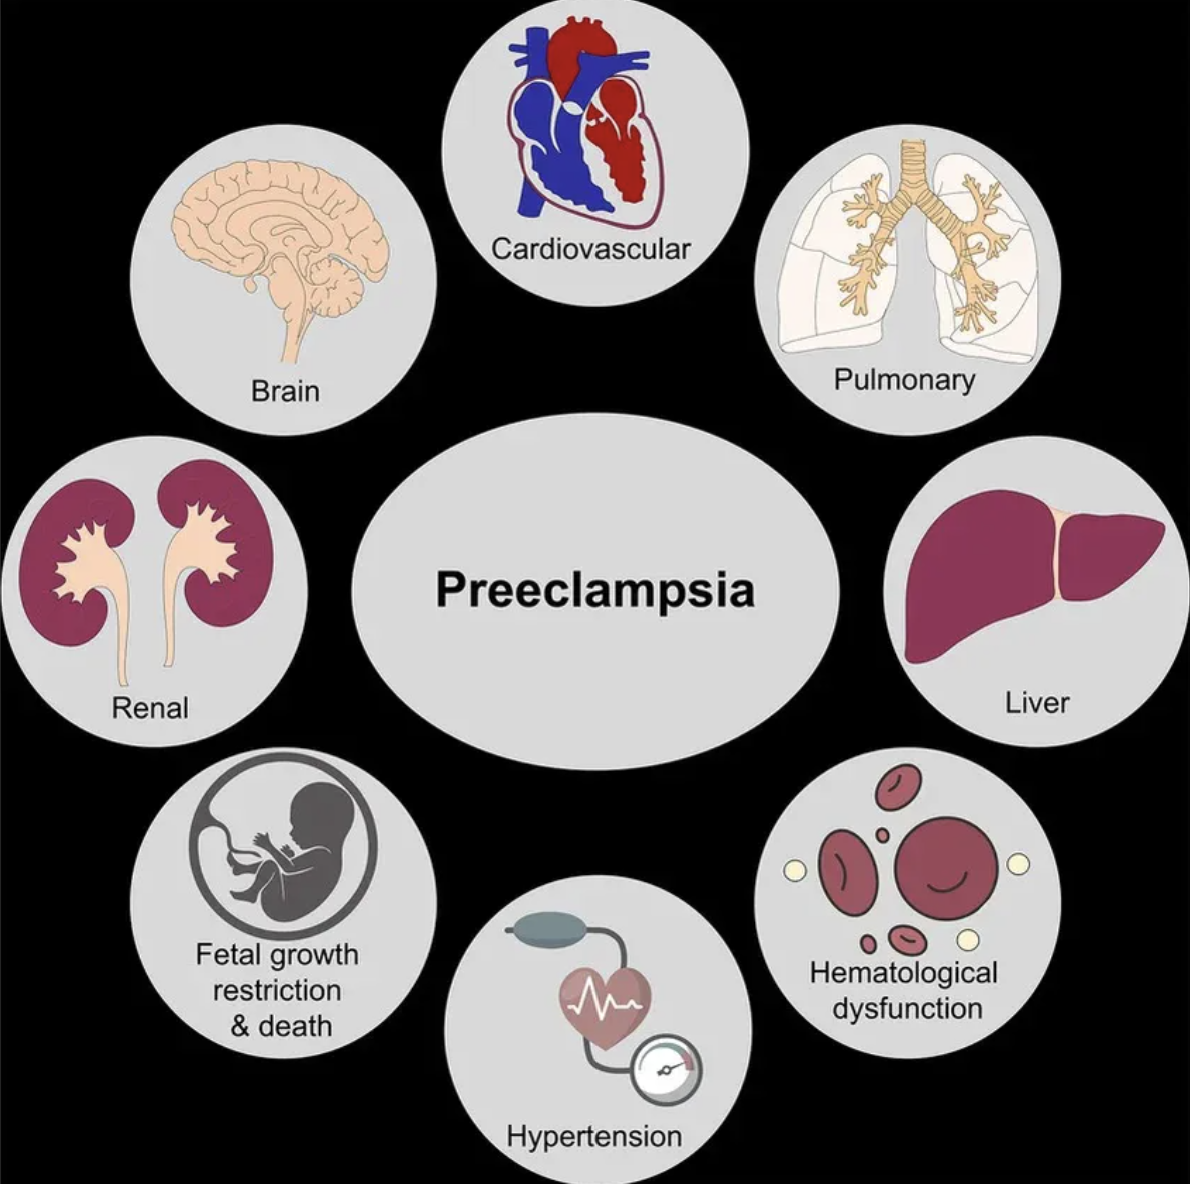
\includegraphics[width=\textwidth]{preeclampsia_infographic.png}
      \end{minipage}
      \hfill
      \begin{minipage}[t]{0.48\textwidth}
        \centering
        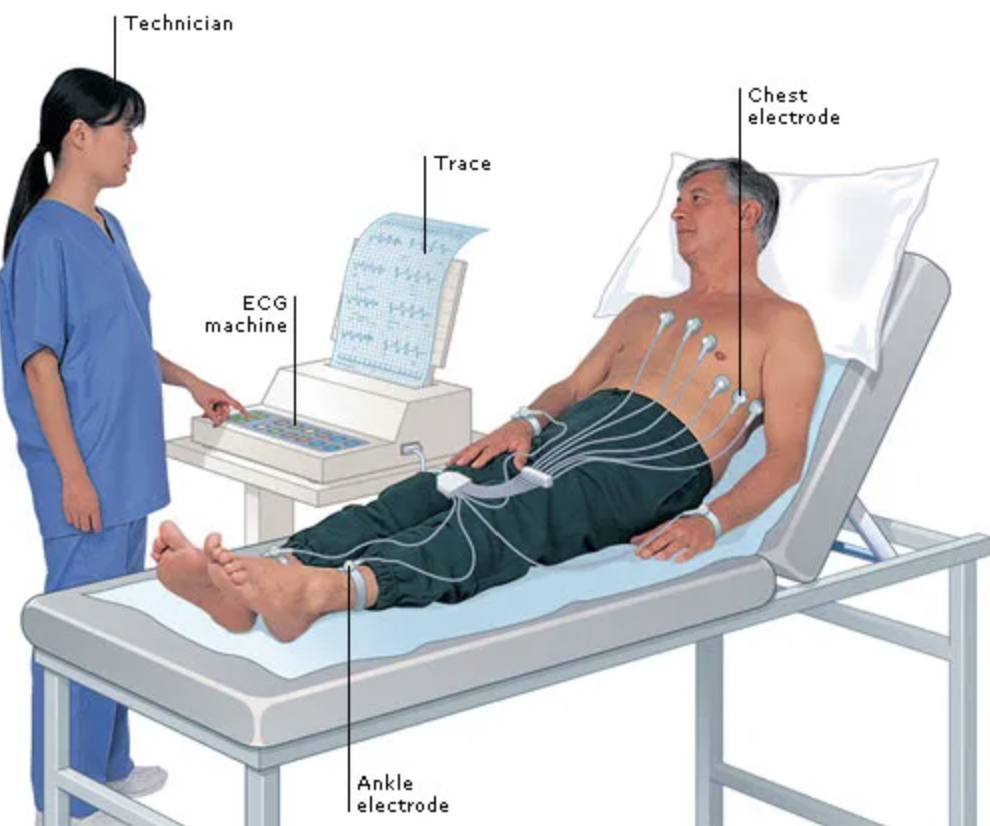
\includegraphics[width=\textwidth]{bed.png}
      \end{minipage}
    \end{column}

    % --- Right Column: Electrode Positioning Diagrams Stacked with Headers ---
    \begin{column}{0.44\textwidth}
      \centering

      % Top Image: Precordial Leads
      \vspace{-1em}
      {\footnotesize\Raleway\color{aggieblue} Precordial Leads}\\[0.2em]
      \begin{center}
        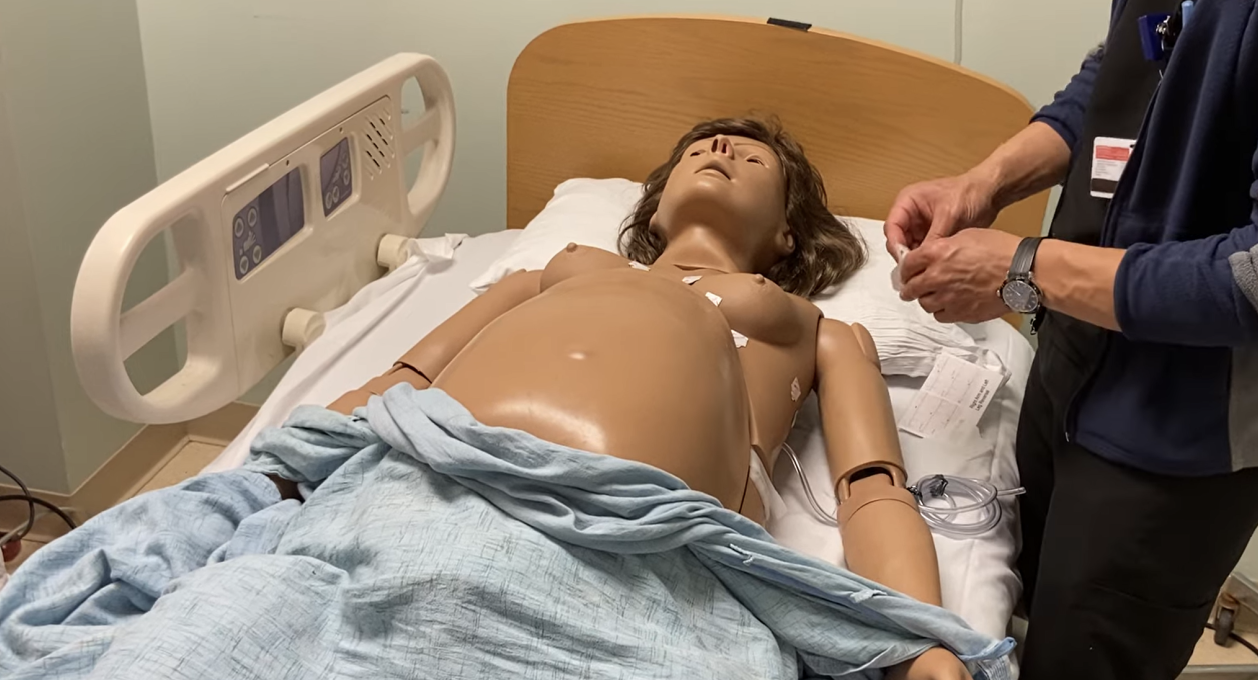
\includegraphics[width=0.8\textwidth]{precordial2.png}
      \end{center}


      % Bottom Image: Limb Leads
      {\footnotesize\Raleway\color{aggieblue} Limb Leads}\\[0.2em]
      \begin{center}
        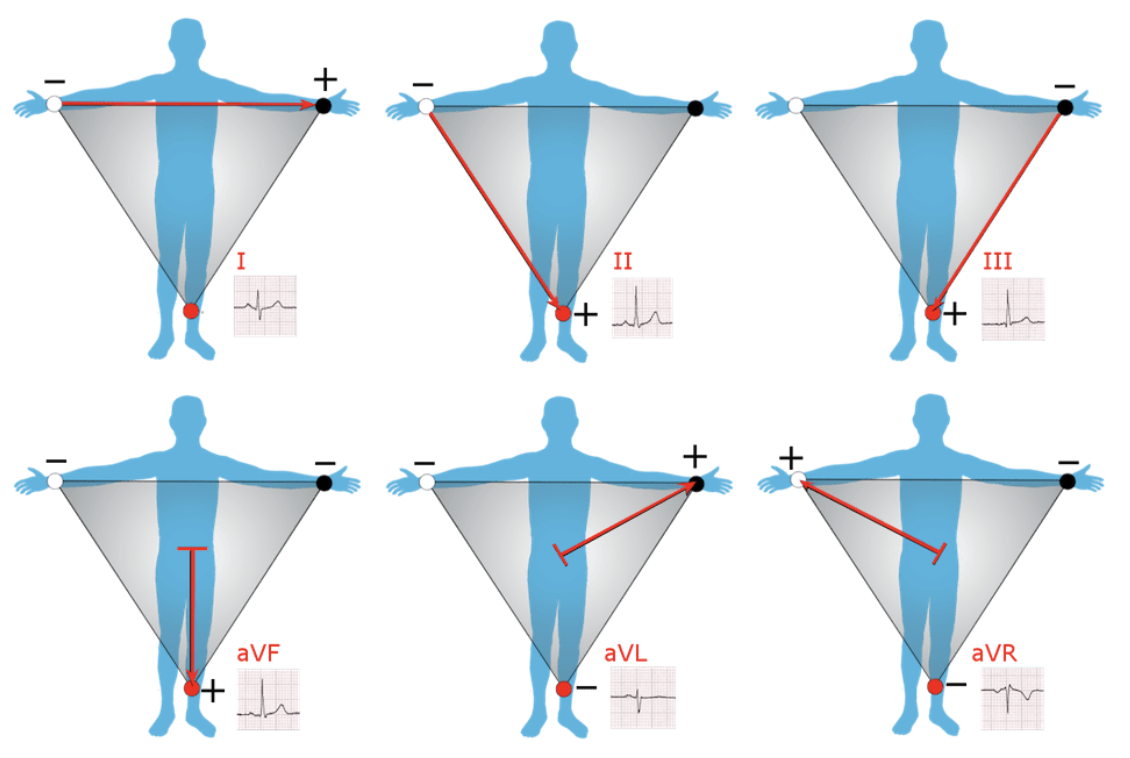
\includegraphics[width=0.75\textwidth]{limb_leads.png}
      \end{center}
    \end{column}

  \end{columns}
\end{frame}

% ---------- Subsection Slide: Dataset Profile ----------
\begin{frame}{Decision-Tree Modeling}
  \begin{columns}[T]

    % Left Column: Fills the vertical space better with larger font
    \begin{column}{0.44\textwidth}
      \centering
      {\small\Raleway\bfseries\color{aggieblue} ECG Dataset Breakdown}\\[1.0em]

      \renewcommand{\arraystretch}{1.5}
      \resizebox{\textwidth}{!}{%
        \begin{tabular}{lccc}
          \toprule
          \textbf{Dataset} & \textbf{\shortstack{Original Total\\(P/N)}} & \textbf{\shortstack{Dropped ECGs\\(P/N)}} & \textbf{\shortstack{Final Total\\(P/N)}} \\
          \midrule
          \textbf{Unbalanced} & 337 / 1854 & 8 / 24 & 329 / 1830 \\
          \bottomrule
        \end{tabular}
      }
      
      \vfill % Pushes content down dynamically to fill space
      
      \begin{flushleft}
      \small\color{coolgray} % Increased from footline font to small
      Each ECG sample includes \textbf{656 distinct MUSE metadata features.}\\[1.2em]

      \textbf{Cross-Validation Strategy:}
      \begin{itemize}
        \setlength{\itemsep}{4pt} % Generous spacing to fill vertical space
        \footnotesize
        \item \textbf{StratifiedGroupKFold} with 5 folds grouped by the Patient's MRN
        \item \textbf{Ensemble} with \textbf{RandomUnderSampler} inside the folds
      \end{itemize}
      \end{flushleft}
    \end{column}

    % Right Column: Adjusted heights and spacing to completely fit the list
    \begin{column}{0.52\textwidth}
      \centering
      {\small\Raleway\bfseries\color{aggieblue} ECG Signal}\\[0.5em]

      \begin{beamercolorbox}[wd=\textwidth,rounded=true,shadow=false,sep=0.1em]{boxgray}
        \centering
        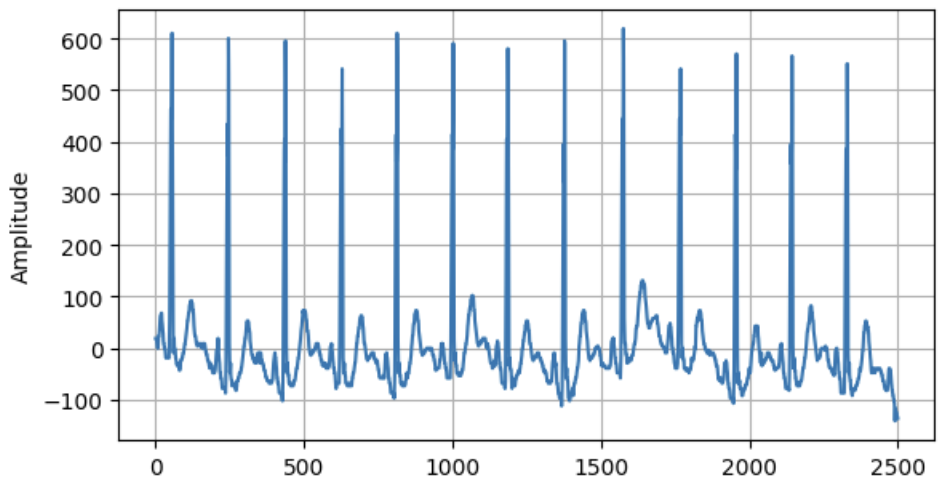
\includegraphics[width=1\textwidth,height=2.1cm,keepaspectratio=false]{v3_pre.png}
      \end{beamercolorbox}

      \vspace{0.6em}
      \begin{flushleft}
      \textbf{Unweighted-Voting Model:}
      \begin{itemize}
        \setlength{\itemsep}{1pt} % Compact spacing to ensure SVM fits perfectly
        \small
        \item \textbf{RandomForest}
        \item \textbf{CatBoost}
        \item \textbf{XGBoost}
        \item \textbf{LightGBM}
        \item \textbf{LogisticRegression}
        \item \textbf{SVM}
      \end{itemize}
      \end{flushleft}
    \end{column}
  \end{columns}
\end{frame}


\begin{frame}{Conclusion \& Future Work}

  % --- TOP SECTION: Model Performance Table ---
  \setlength{\tabcolsep}{5pt}
  \vspace{-0.3em}
  \centering

  {\small\Raleway\bfseries\color{aggieblue} Model Performance}\\[0.2em]
  \begin{beamercolorbox}[wd=\textwidth,rounded=true,shadow=false,sep=0.3em]{boxgray}
    \small % Bumped table font size up from \tiny to \small
    \resizebox{\textwidth}{!}{%
      \begin{tabular}{lcccccc}
        \textbf{Model} & \textbf{AUROC} & \textbf{AUPRC} & \textbf{Specificity} & \textbf{Sensitivity} & \textbf{Balanced Accuracy} & \textbf{F1-Score} \\
        \hline
        Unweighted Voting+ & $75.72 \pm 3.94$ & $41.58 \pm 8.03$ & $74.64 \pm 4.70$ & $62.35 \pm 10.93$ & $68.50 \pm 3.22$ & $40.85 \pm 2.24$ \\
        Neural Network     & $70.9 \pm 4.9$   & $34.2 \pm 7.5$    & $62.7 \pm 12.6$ & $73.0 \pm 9.2$  & $0.00 \pm 0.00$   & $40.4 \pm 6.9$ \\
      \end{tabular}%
    }
  \end{beamercolorbox}

  \vspace{0.6em}

  % --- BOTTOM SECTION: Future Work Split Columns ---
  \begin{columns}[T]

    % Left Column: Shifted to \small for headers and \footnotesize for bullets
    \begin{column}{0.45\textwidth}
      \raggedright
      {\large\Raleway\bfseries\color{black} Future Improvements}\\[0.4em]
      \begin{itemize}
        \setlength{\itemsep}{0.3em}
        \normalsize
        \item Larger, multi-site datasets
        \item Temporal analysis
        \setlength{\itemsep}{0.3em}
        \item Lightweight deployment (fewer leads)
      \end{itemize}
    \end{column}

    % Right Column: Text size increased, graphics scaled down to make room
    \begin{column}{0.51\textwidth}
    \vspace{-0.4em}
      \raggedright 

      % Top Row: Callout text (bumped to \small) and thermometer
      \begin{minipage}[c]{0.65\textwidth}
        \raggedright
        \small\Lato\color{black}\bfseries % Increased to a highly visible \small
        End Goal: Make ECG diagnoses as easy and available as a thermometer!
      \end{minipage}%
      \hfill
      \begin{minipage}[c]{0.30\textwidth}
        \centering
        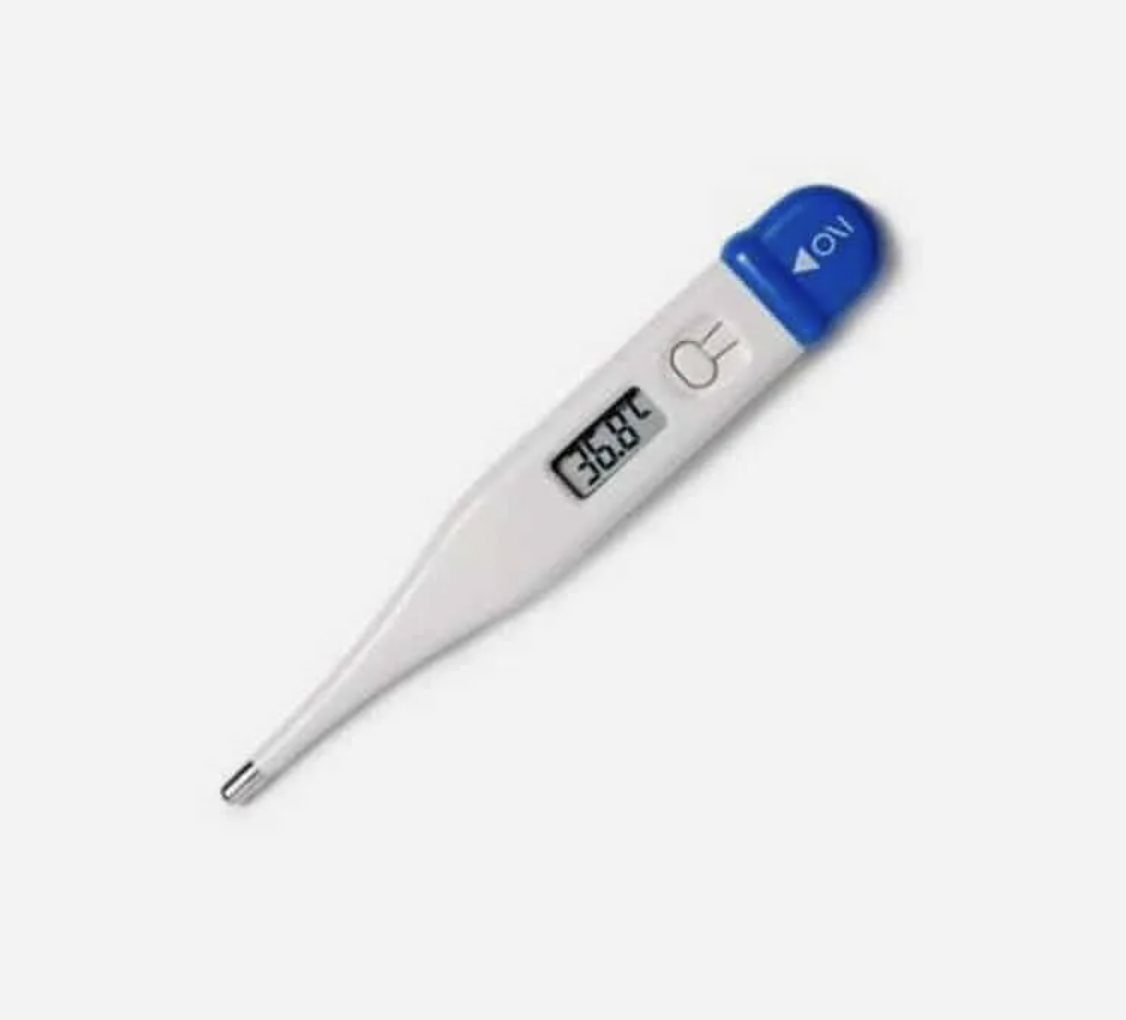
\includegraphics[width=\textwidth]{thermometer.png}
      \end{minipage}

      % Bottom Row: ECG machine print graphic
      \vspace{0.6em}
      \centering
      {\scriptsize\Raleway\bfseries\color{aggieblue} 6 Lead Progression Results}\\[0.3em]
      \begin{beamercolorbox}[wd=\textwidth,rounded=true,leftskip=0.2em,rightskip=0.2em,sep=0.4em]{boxgray}
        \small
        \resizebox{\textwidth}{!}{
          \begin{tabular}{lcc}
            \textbf{Metric} & \textbf{12 Leads} & \textbf{6 Leads} \\
            \hline
            Balanced Accuracy & $64.4\% \pm 11.3\%$ & $63.0\% \pm 7.7\%$ \\
            Precision & $0.66 \pm 0.18$ & $0.64 \pm 0.13$ \\
            Recall & $0.61 \pm 0.16$ & $0.60 \pm 0.13$ \\
            F1 Score & $0.62 \pm 0.14$ & $0.61 \pm 0.11$ \\
            ROC-AUC & $0.64 \pm 0.11$ & $0.63 \pm 0.08$ \\
          \end{tabular}
        }
      \end{beamercolorbox}
      
    \end{column}

  \end{columns}
\end{frame}
% ---------- Closing Slide ----------
{%
  \setbeamertemplate{footline}{}%
  \begin{frame}[plain,noframenumbering]
    \begin{tikzpicture}[remember picture,overlay]
      \fill[aggieblue] (current page.south west) rectangle (current page.north east);
    \end{tikzpicture}
    \vfill
    \centering
    {\Raleway\bfseries\Huge\color{white} Thank you}\\[0.6em]
    {\color{aggiegold}\rule{4cm}{0.06cm}}\\[0.8em]
    \vfill
  \end{frame}
}

\end{document}